%TODO: move this chapter as a section to introduction and add here the new "Problem statement" chapter!!!

\chapter{Memory model-aware analysis}%Description of the analysis of concurrent systems wrt weak memory models
%\chapter{A generic framework}
\label{ch:wmm}

In general, analysis of concurrent programs with respect to axiomatic memory models is performed in several stages. %TODO: site the 'Weak Memory Models with Matching Axiomatic and Operational Definitions' https://arxiv.org/pdf/1710.04259.pdf
%TODO: cite also: "DENNIS SHASHA - Efficient and Correct Programs that Share" http://citeseerx.ist.psu.edu/viewdoc/download?doi=10.1.1.142.2238&rep=rep1&type=pdf
Firstly, the control-flow and data-flow of a program is encoded as the set of possible \textit{candidate executions}. %possible communications between threads of the program.
Obtained model of the program describes the anarchic semantics, which is a truly parallel semantics with no global time that describes all possible computations with all possible communications~\cite{alglave2016syntax}. Thereafter, the anarchic semantics is constrained by the \textit{weak memory model} specification which is a set of axiomatic constraints for filtering out executions inconsistent in particular architecture.


\section{The event-based program representation}
\label{ch:wmm:event}

%"The semantics of a program is a set of executions" https://johnwickerson.github.io/papers/memalloy.pdf
The classical approach for modeling concurrent programs is to use the \textit{global time}, a single order of interleavings among all events happened in different threads.
Although these models are easy to understand, it may be impossible to treat \textit{all} possible states, number of which is exponentially large.
However, there exist equivalence classes such that the result of execution different interleavings from single equivalence class is the same (for instance, computations performed by a processor locally do not affect the global state).
%One way to do this is to use a non-deterministic computation-centric model~\cite{fri97}, such as ...%The idea in this class of models is based on the fact that the behaviour of a concurrent system is defined only by the interleavings of shared-memory operations, while being independent from the order of local computation events.
%TODO: nondeterministic
One such model is the \textit{event-based} representation of a program, which models a program as a directed graph of events (the \textit{event-flow graph}).
The vertices of such a graph represent \textit{events} (see Section~\ref{ch:wmm:model:events}), and edges represent \textit{basic relations} (see Section~\ref{ch:wmm:model:relations}).

% TODO: the event-based representation is a non-deterministic model

% TODO: the semantics of the event-flow graph is given:  "alglave: Don’t sit on the fence A static analysis approach to automatic fence insertion" page 8 or 9
%"To build the aeg , we define a semantics of goto-programs in terms of abstract events, ..."
% TODO: OR from here: http://www.cprover.org/etaps/esop.pdf "Software Verification for Weak Memory via Program Transformation"

\subsection{Events}
\label{ch:wmm:model:events}

%TODO: event is atomic?

% TODO: check this subseciton

The event is an independent low-level atomic operation.

A \textit{memory event} $e_m \in \mathbb{E}$ represents the fact of access to the memory.
Only memory events change the state of an abstract machine executing the code, since it is completely determined by values stored in its memory.
Since memory is the crucial low-level resource shared by multiple processes, most relations are defined over memory events. 
The processes can access a shared memory location (denoted by~$l_i$, for \textit{location}), or a local one (denoted by~$r_i$, for \textit{register}).
A memory event can access at most one shared memory location, high-level instructions that address more than one shared variable must be transformed into a sequence of events.
A memory event is specified by its direction with respect to the shared variable, its location~$\mathtt{loc}(e_m)$, its processor label~$\mathtt{proc}(e_m)$, and a unique event label~$\mathtt{id}(e_m)$~\cite{alglave2010shared}.
%\texttt{load} for read the value of a shared-memory location, or \texttt{store} for write, or neither of them if both locations are local

The set of memory events $\mathbb{M}$ is divided into write events $\mathbb{W}$ (that write values to shared-memory locations) and read events $\mathbb{R}$ (that read values stored in shared-memory locations).
We add a restriction that each memory event uses at most one shared location, so that the write instruction $i = write(l_1, l_2)$, that encodes the write from the shared location $l_2$ to the shared location $l_1$, is represented as two consequent events $e_1~=~\mathtt{load}(r_1~\leftarrow~l_2); \ e_2~=~\mathtt{store}(l_1~\leftarrow~r_1)$.
Also, it is important to separate the set of initial write events $\mathbb{IW}~\subset~\mathbb{W}$ that perform initialisation of program variables.

A \textit{computation event} $e_c \in \mathbb{C} \subseteq \mathbb{E}$, represents a low-level assembly computation operation performed solely on local-memory arguments.
An example of computation event may be the event $e_c = r_1 \leftarrow add(r_2, 1)$ that writes the sum of values stored in register $r_2$ and constant $1$ (which is modelled as a register as well) to the register $r_1$.
For modelling branching statements, we distinguish the set $\mathbb{C_{p}}~\subseteq~\mathbb{C}$ of \textit{predicative} computation events (also called as \textit{branching events}), that are evaluated as a boolean value.

The synchronisation instructions (fences) cause the \textit{barrier events}, that do not perform any computation or memory value transfer, instead, they add new relations to the program model that restrict the set of allowed behaviours.
Functionally, a fence may be a synchronisation barrier or a instruction of flushing the local memory caches, etc.

% TODO: more fences: "On Power and ARM (see Sec. 6), we distinguish between control fence (which we write cfence), lightweight fence (lwfence) and full fence (ffence). On x86, implementing TSO, there is only one fence, called mfence." (herding cats, p. 14)

\subsection{Relations}
\label{ch:wmm:model:relations}

%In this section, we describe basic relations used in memory model-aware program analysis.

The relation~%\xrightarrow{r}
$r\,\subseteq~\mathbb{E}~\times~\mathbb{E}$ is a set of pairs of events (a subset of Cartesian product of two sets of events). There are two kinds of relations between events: \textit{basic relations} %retrieved from the 
that capture semantics of the program, and \textit{derived relations} that are defined from the basic relations and events in the weak memory model specification. Constraints over relations that are specified by weak memory models are defined as requirements of acyclicity, irreflexivity or emptiness of specific relations~\cite{alglave2016syntax}.

\vspace{1em}
The basic relations are the following~\cite{alglave2010shared}:
%TODO: say that po and rf are  defined from the candidate execution:
%TODO: say that 
\begin{itemize}
    \item The \textit{control-flow} of a program is defined by the \textit{program-order} relation \po~$\subset~\mathbb{E}~\times~\mathbb{E}$, which represents the total order of events of same process.
    For instance, if the instruction $i_1$ generates the event $e_1$ and the instruction $i_2$ follows $i_1$ and generates the event $e_2$, then $e_1 \relation{po} e_2$.
    %Some new relations may be acquired : dp, po-loc

    \item The \textit{data-flow} of a program is defined by \textit{communication relations}:
        \begin{itemize}[noitemsep]
            \item the \textit{read-from} relation \rf~$\subset~\mathbb{W}~\times~\mathbb{R}$ that maps each write event to the read event that reads the value written by write event;
            \item the \textit{coherence order} relation \co~$\subset~\mathbb{W}~\times~\mathbb{W}$ that defines the total order on writes to the same location across all processes (also called the \textit{write serialisation}, \texttt{ws}-relation);
        \end{itemize}

    \item Events from the same process are related by the \textit{scope relation} \sr~$\subset~\mathbb{E}~\times~\mathbb{E}$.
    In contrast to the \tool{herd} tool, the \porthos[2] does not use hierarchy of scopes (depicted as the scope tree); instead, it uses simple lables that indicate which process has produced certain event.
\end{itemize}

%TODO: add ppo = characteristics of memory model. "Architectures are instances of our model. An architecture is a triple of functions (ppo, fences, prop), which specifies the preserved program order ppo, the fences fences and the propagation order prop." (herding cats, p.13)

Below we enumerate some derived relations~\cite{alglave2010shared}:

\begin{itemize}

    \item the \textit{from-read} relation $\fr \subset~\mathbb{R}~\times~\mathbb{W}$ that maps a read event to all write events preceding the write event from which the read event gets its value: \\
    $r \relation{fr} w ~\triangleq~ (\exists w' . w' \relation{rf} r \land w' \relation{co} w)$

    %\item the \textit{data dependency} relation \texttt{dp}, which is a subset of \po-relation that always has a read at its source (it connects the read to the write which it depends on)
    %TO-DO: formula for dp or exclude

    \item the \textit{communication} relation \com over memory events, that fully describes the data-flow of a program: \\
    %$\mathtt{com} \triangleq (\mathtt{rf} \cup \mathtt{co} \cup \mathtt{fr})$
    $m_1 \relation{com} m_2~\triangleq~((m_1\relation{rf}m_2) \lor (m_1\relation{co}m_2) \lor (m_1\relation{fr}m_2))$

    \item the \textit{external} (and \textit{internal}) \textit{read-from} relations that restrict the \rf-relation to the different (respectively, same) processes: \\
    $w \relation{fre} r ~\triangleq~ (w \relation{fr} r \land \mathtt{proc}(w) = \mathtt{proc}(w))$ \\
    $w \relation{fri} r ~\triangleq~ (w \relation{fr} r \land \mathtt{proc}(w) \neq \mathtt{proc}(w))$
    
    %TODO: say that po-relation is *static*
    \item the \texttt{po-loc} relation that is the \po-relation over events that access to the same shared variable: \\
    $m_1 \relation{po-loc} m_2 ~\triangleq~ (m_1 \relation{po} m_2 \land \mathtt{loc}(m_1) = \mathtt{loc}(m_2))$

    \item the semantics of \textit{fences} (memory barriers) specific for different architectures may be defined as derived relations.

    %"Preserved program order defines the set of reorderings guaranteed by the architecture not to occur, based on the types of the accesses." http://delivery.acm.org/10.1145/2750000/2742219/p635-lustig.pdf

\end{itemize}

%todo: some words here?


\subsection{Executions}
\label{ch:wmm:model:executions}

The semantics of a concurrent program is represented as the set of allowed executions. The 
The \textit{execution} is a path in the event-flow graph defined by \po- and \rf-relations and set of final writes to a given memory location that is valid under certain memory model~\cite{alglave2014herding}.
It can be interpreted as a sequence of guesses which event is to be executed next.
The \textit{candidate execution} is an execution that is not yet constrained by a memory model.

%TODO: cite this paper elsewhere
%As it was shown in~\cite{wickerson2017automatically}, it is enough for memory models to constrain the executions independently instead of constraining the program at a whole.

%An \textit{execution} (trace, run) of a program is an ordered set of events defined by \po- and \rf-relations and set of final writes to a given memory location that is valid under certain memory model~\cite{alglave2014herding}.
%The order of events in particular execution is denoted as `$\rightarrow$', an empty execution is denoted as $\emptyset$.
%associated with the instructions of the program
%An execution is considered to be \textit{valid} if the memory events follow a single global timeline, i.e., can be embedded in a single partial order allowed by the memory model restrictions~\cite{alglave2010shared}.
%An execution is uniquely defined by the set $\mathbb{X}$ of events have been executed in each thread (the \textit{control-flow} of a program), and the relations $\mathtt{rf}$ and $\mathtt{co}$~\cite{alglave2010shared}.
Figure~\ref{simple_wmm_x86_pic} illustrates four possible candidate executions for the litmus test Example~\ref{simple_wmm_x86} (the pictures are generated by the \tool{herd7} tool, version~7.47).
Since there are no conditional jumps, the \po-relation is defined and we do not need to guess it.
Since each thread performs single write followed by a single read, the \co-relation is also defined (it relates the initial write event with the write event to the same location).

\begin{figure}[!htb]
\centering
\begin{subfigure}[t]{.28\textwidth}
  \centering
  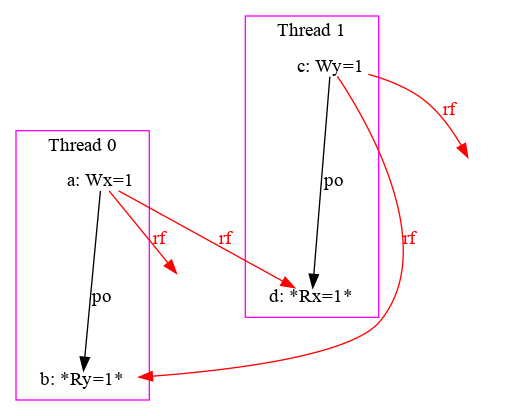
\includegraphics[width=1.2\linewidth]{img/my/sb-example/SB-dot.png}
  \caption{Final state: \texttt{(0:EAX=1~/\textbackslash~1:EAX=1)}}
  \label{simple_wmm_x86_pic:sub1}
\end{subfigure}
\hfill
\begin{subfigure}[t]{.23\textwidth}
  \centering
  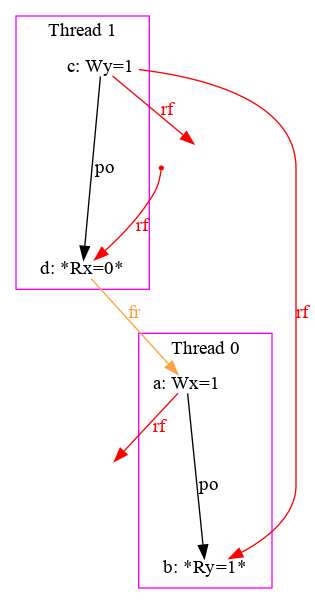
\includegraphics[width=.9\linewidth]{img/my/sb-example/SB-dot-2.png}
  \caption{Final state: \texttt{(0:EAX=1~/\textbackslash~1:EAX=0)}}
  \label{simple_wmm_x86_pic:sub2}
\end{subfigure}
\hfill
\begin{subfigure}[t]{.23\textwidth}
  \centering
  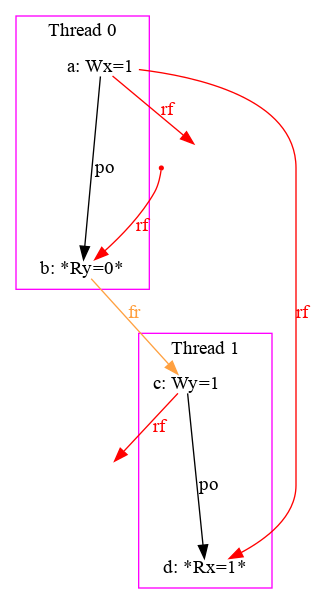
\includegraphics[width=.9\linewidth]{img/my/sb-example/SB-dot-3.png}
  \caption{Final state: \texttt{(0:EAX=1~/\textbackslash~1:EAX=1)}}
  \label{simple_wmm_x86_pic:sub3}
\end{subfigure}
\hfill
\begin{subfigure}[t]{.23\textwidth}
  \centering
  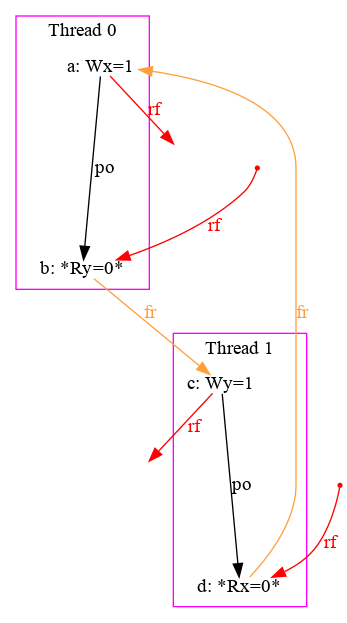
\includegraphics[width=.9\linewidth]{img/my/sb-example/SB-dot-4.png}
  \caption{Final state: \texttt{(0:EAX=0~/\textbackslash~1:EAX=0)}}
  \label{simple_wmm_x86_pic:sub4}
\end{subfigure}
\hfill
\caption{Possible candidate executions for the litmus test Example~\ref{simple_wmm_x86}}
\label{simple_wmm_x86_pic}
\end{figure}

Thus, there are only four possible executions defined by the choice of \rf-relation.
The candidate executions pictured in Figures~\ref{simple_wmm_x86_pic:sub1}--\ref{simple_wmm_x86_pic:sub3} are consistent both under strong memory model SC and under relaxed memory models x86-TSO, Power, ARM, and some others.
However, the execution shown in Figure~\ref{simple_wmm_x86_pic:sub3} is still consistent under relaxed-memory architectures, but it becomes inconsistent under SC architecture as it forbids cycles over~$\fr\cup\po$.
%However, the Power memory model allows such cycles, therefore %TODO: include load buffering example, see presentation pdf


\section{The \cat{} language}
\label{ch:wmm:cat}

Weak memory models are defined via the \cat{} language~\cite{alglave2016syntax}.
This is a domain specific language for describing consistency properties of concurrent programs.
The \cat{} language combines expressive power of a functional language (it is inspired by OCaml and adopts its types, first-class functions, pattern matching and other features) with types, operations and assertions that are specific for operating with relations and executions.
%represents the functional language extended by the theory of  allows to axiomatically define derived relations, architecture-specific fences, and constraints over relations.
In \cat{}, new relations can be defined via the keyword \texttt{let} and the following operators over relations~\cite{alglave2016syntax}. % 3.1.6 Relations between events

%TODO: this is binary relations. ADD UNARY RELS!

Below we enumerate pre-defined operators over relations and sets of events:

\begin{enumerate}
  \item \textit{Unary relations}:
    \begin{itemize}
      \item \textit{the complement} of a relation \rel{r} is $\rel{\textasciitilde r}$
      \item \textit{the transitive closure} of a relation \rel{r} is $\rel{r+}$
      \item \textit{the reflexive closure} of a relation \rel{r} is $\rel{r?}$
      \item \textit{the reflexive-transitive closure} of a relation \rel{r} is $\rel{r*}$
      \item \textit{the inverse} of a relation \rel{r} is $\invrel{r}$
    \end{itemize}
  \item \textit{Binary relations:}
  \begin{itemize}
    \item \textit{the union} of two relations \rel{r1} and \rel{r2} is \rel{r1\,|\,r2}
    \item \textit{the intersection} of two relations \rel{r1} and \rel{r2} is \rel{r1\,\&\,r2}
    \item \textit{the difference} of two relations \rel{r1} and \rel{r2} is $\mathtt{r1\,\backslash\,r2}$
    \item \textit{the sequence}\footnote{The sequence of two relations \rel{r1} and \rel{r2} is defined as the set of pairs \rel{(x,y)} such that there exists an intervening \rel{z}, such that $\rel{(x,z)} \in \rel{r1}$ and $\rel{(z,y)} \in \rel{r2}$}
    of two relations \rel{r1} and \rel{r2} is \rel{r1;r2}
  \end{itemize}
\end{enumerate}

For instance, the \fr-relation is defined as a sequence of inverted \rf-relation and \co-relation: $\mathr{fr} = (\mathr{rf}^{-1};\mathr{co})$. As an example memory model definition in \cat{} language, the the x86-TSO can be found in Appendix~\ref{apx:x86cat}. This memory model asserts acyclicity of communication relation, \rel{po-loc} relation, \rel{mfence} relation and some other derived relations~\cite{owens2009better}.
